\documentclass[10pt,a4paper,table,xcdraw]{article}

\counterwithin{figure}{section}

\addtolength{\oddsidemargin}{-.5in}
\addtolength{\evensidemargin}{-.5in}
\addtolength{\textwidth}{1in}
\addtolength{\topmargin}{-.5in}
\addtolength{\textheight}{1in}

\usepackage{caption}
\usepackage{subcaption}
\usepackage{graphicx}
\usepackage{wrapfig}
\graphicspath{{images/}}
\usepackage{pgf-pie}
\usepackage{pdfpages}

% Math
\usepackage{amssymb}
\usepackage{amsmath} % Required for some math elements

% Other
\usepackage{algorithmic}
\usepackage{array}
\usepackage{lipsum}
\usepackage{pgfplots}
% \usepackage{hyperref}
\usepackage{caption}
\usepackage{float}
\usepackage{tikz}
\usetikzlibrary{snakes}
\usepackage{rotating}

% tables
\usepackage{booktabs}
\usepackage{multirow}
\usepackage{titlesec}

\usepackage{parskip}
\usepackage[toc,page]{appendix}
\usepackage[hidelinks]{hyperref}

\usepackage[normalem]{ulem}
\useunder{\uline}{\ul}{}
\usepackage{tocloft}

\addtolength{\cftsecnumwidth}{10pt}

\newenvironment{conditions}
  {\par\vspace{\abovedisplayskip}\noindent\begin{tabular}{>{$}l<{$} @{${}={}$} l}}
  {\end{tabular}\par\vspace{\belowdisplayskip}}

% Define section numbering style
\renewcommand{\thesection}{\Roman{section}} % Capital Roman numerals for sections
\renewcommand{\thesubsection}{\Alph{subsection}} % Capital letters for subsections
\renewcommand{\thesubsubsection}{\roman{subsubsection}} % Lowercase Roman numerals for subsubsections

\usepgfplotslibrary{external}
\tikzexternalize

\pgfplotsset{compat=1.18}

\begin{document}

\title{DECA Sales Project} % Title
\author{(in order of importance and reverse height) Nathan Dai, Lynn Huang, Ruby Gao}
% \date{\today} % Date for the report
\date{February 2024} % Date for the report
\maketitle % Inserts the title, author and date

\clearpage
\setcounter{tocdepth}{4}
\tableofcontents
\clearpage

\section{Executive Summary}

One- to three-page description of the project

\section{Initiating}

\subsection{Problem Statement}

Statement of the problem

\subsection{Project Scope}

Project scope — brief description of the project (purpose, rationale and expected benefits)


\section{Planning and Organizing}

\subsection{Project Goals}

Project Goals

\subsection{Human Resource Management Plan}

Human resource management plan — team member roles, skills and strengths, and responsibilities

\subsection{Schedule}

\subsubsection{Milestone}

Milestone — describe the 2-4 major milestones (activities) needed to accomplish

\subsubsection{Timeline}

Timeline to reach each milestone


\subsection{Quality Management Plan}

Quality management plan — key metrics

\subsection{Risk Management Plan}

\subsubsection{Overall Risk: Insufficient Attendance}

The primary risk we identified in our carnival planning is the potential for insufficient attendance. This overarching risk could have significant implications, including financial loss due to the cost of running the event exceeding the revenue generated, and damage to DECA's brand image if attendees perceive poor value for money.

To mitigate this overall risk, we have identified and addressed several interconnected risks. These include the risk of lack of interest leading to low attendance, for which we have implemented a robust advertising campaign and collaborated with teachers to offer extra credit incentives. We also considered the risk of attendees perceiving poor value for money, and have committed to maintaining transparency in all dealings. Finally, we have strategies in place to address the risk of inadequate advertising and engagement hindering a successful promotion of the event.

By addressing these interconnected risks, we aim to ensure a successful carnival with high attendance, positive attendee experiences, and a strengthened DECA brand image.


\subsubsection{Risk 0: Carnival Mis-Scheduling}

Given the busy schedules of CCA students, there is a potential risk that the chosen date and time may not be convenient for all students, leading to lower attendance. The potential impact of this risk is significant. Lower attendance could lead to reduced ticket sales, less engagement, and a less successful event overall.

To mitigate this risk, we have carefully considered the timing of the carnival. We chose a Friday afternoon, a time when students are likely to be more available and less reluctant to stay after school due to the absence of tests or homework due the next day. We also strategically avoided scheduling the carnival on the Friday of finals week, recognizing that students would be too focused on their exams to attend our event. Additionally, we avoided dates when early decision results from universities are released, as this could be a stressful time for many seniors.

By carefully considering the scheduling of the carnival, we aim to maximize attendance and ensure the success of the event.


\subsubsection{Risk 1: Misestimation of Ticket Distribution}

\begin{table}[H]
	\centering
	\caption{Early bird pricing model}
	\begin{tabular}{r|rr|rr}
	\multicolumn{1}{l|}{\textbf{Tickets}} & \multicolumn{1}{l}{\textbf{Price / Ticket (\$)}} & \multicolumn{1}{l|}{\textbf{Price (\$)}} & \multicolumn{1}{l}{\textbf{Early Discount (\%)}} & \multicolumn{1}{l}{\textbf{Early Price (\$)}} \\ \hline
	1                                     & \$ 1.00                                          & \$ 1.00                                  & 0\%                                              & \$ 1.00                                       \\
	5                                     & \$ 0.90                                          & \$ 4.50                                  & 6\%                                              & \$ 4.25                                       \\
	10                                    & \$ 0.80                                          & \$ 8.00                                  & 13\%                                             & \$ 7.00                                       \\
	20                                    & \$ 0.75                                          & \$ 15.00                                 & 17\%                                             & \$ 12.50                                      \\
	50                                    & \$ 0.50                                          & \$ 25.00                                 & 20\%                                             & \$ 20.00
	\end{tabular}
	\label{tab:ticket_pricing}
\end{table}

\autoref{tab:ticket_pricing} shows how the price per ticket changes as the number of tickets bought increases as well as the early-bird discount. The ticket pricing strategy we employed incorporated a quantity discount model, which offers a lower cost per ticket when purchased in larger quantities. Additionally, we implemented an early bird pricing model, providing a discount for tickets purchased in advance.

\begin{table}[H]
	\caption{Estimated ticket distribution. The count represents the percentage of people who bought that number of tickets. For example, we estimate that 40\% of people will buy 1 ticket.}
	\begin{tabular}{r|rr}
	\multicolumn{1}{l|}{\textbf{Tickets}} & \multicolumn{1}{l}{\textbf{Count (\%)}} & \multicolumn{1}{l}{\textbf{Price / Ticket (\$)}} \\ \hline
	1                                     & 40\%                                    & \$ 1.00                                          \\
	5                                     & 25\%                                    & \$ 0.90                                          \\
	10                                    & 20\%                                    & \$ 0.80                                          \\
	20                                    & 12\%                                    & \$ 0.75                                          \\
	50                                    & 3\%                                     & \$ 0.50
	\end{tabular}
	\label{tab:estimated_ticket_distribution}
\end{table}

We also estimated the distribution of ticket purchases, as shown in \autoref{tab:estimated_ticket_distribution}. This estimation was based on surveys conducted among a random selection of individuals from our classes. Their responses were factored into the final estimate. Consequently, we calculated the estimated average price per ticket to be \$0.75.

It is important to note that while estimating the average price per ticket, we did not consider the early bird discount. This discount was primarily intended for friends of the carnival game operators, and we do not anticipate a significant portion of total ticket sales to be early bird sales.


\subsubsection{Risk 2: Not Enough Game Operators}

At our school, the AP Statistics class each year completes a carnival project, where they learn about expected values. Each group designs a game where they are expected to earn fake money from their game on the culminating Carnival Day, where students are given fake money to play the games. We are recruiting these students to be the game operators at our carnival because they have already designed games where they are expected to win.

In our strategic planning for the carnival, we identified a potential risk associated with our profit-sharing model for game operators. Given that the game operators were only entitled to 30\% of the profits they generated, there was a concern that this might not be a sufficient incentive for a large number of students to sign up as operators. This risk was further compounded by the fact that we, as the organizers, were absorbing all the financial risks associated with the event, including the upfront costs of the prizes.

The potential impact of this risk was significant. If we were unable to recruit a sufficient number of game operators, we would not have enough games at the carnival. This could lead to a less engaging and enjoyable experience for attendees, potentially impacting ticket sales and overall success of the event.

To mitigate this risk, we implemented a multi-faceted strategy. Firstly, we worked closely with the AP Statistics teachers to encourage more students to sign up as game operators, leveraging the alignment of the carnival project with their curriculum and emphasizing the little effort it would take to set up their previously made game. Secondly, we emphasized the non-financial benefits of participating as a game operator, such as the opportunity to apply their classroom learning in a real-world context, and the enjoyment of being part of a school-wide event. Lastly, we offered additional incentives such as complimentary food and beverages for game operators. Through these measures, we aimed to ensure a sufficient number of game operators to make the carnival a success.


\subsubsection{Risk 3: Disincentivized Players}

A significant risk we identified pertains to the incentivization of play. The carnival games we selected from the AP Statistics class are designed to statistically favor the game organizer. While individual play involves an element of chance, the Law of Large Numbers dictates that the probability of the game operator incurring a loss decreases as the number of players increases [\ref{appendix:large_numbers}].

However, a considerable portion of our carnival attendees were friends who were aware that the games were skewed in favor of the operators. We were concerned that this knowledge might deter participation. The potential impact of this risk was substantial, as reduced player engagement could lead to lower ticket sales and diminished overall enjoyment of the carnival.

To mitigate this risk, we conducted research into the economics of various gambling institutions and discovered the favorite-longshot bias. This well-documented phenomenon reveals that people often overestimate the impact and likelihood of extremely low-probability events [\ref{appendix:favorite_longshot}]. We concluded that individuals are drawn to risk when it is accompanied by the potential for substantial returns. Thus, in a gambling transaction, both the bettor and the bet acceptor find their actions worthwhile. Our carnival benefits by generating overall profits, while participants derive enjoyment from the prospect of winning a large prize.

Furthermore, it is improbable that an individual would discern that our carnival games are designed to favor the operators purely through playing the game. Each player can attribute their losses to random chance, while we, as the organizers, have a broader perspective. This understanding informed our risk mitigation strategy, ensuring that our carnival remains both profitable and enjoyable for all participants.


\subsubsection{Risk 4: Prize Manipulation}

A potential risk we identified in our carnival planning pertains to the game operators' incentive structure. Given that the game operators bear no financial risk, they may not be sufficiently motivated to limit prize giveaways. This situation could potentially lead to collusion between game operators and their friends, resulting in our prizes being obtained at a lower cost.

The potential impact of this risk is significant. If unchecked, such collusion could lead to financial loss for the carnival and undermine the fairness of the games, potentially impacting the overall success of the event.

To mitigate this risk, we implemented a robust detection and prevention strategy. During the sign-up process, game operators provide us with the theoretical probabilities of each game outcome and the prizes associated with each category. We then calculate the expected profit of their game, ensuring it is not excessively low. We anticipate that the expected profit may be low for many games, as it is calculated using the cost of the prize, while the perceived value of the prize may be much higher.

Post-carnival, each game operator is required to produce a log detailing the number of times each outcome (lose, small, medium, large) occurred. We employ a Chi-Square Goodness of Fit Test [\ref{appendix:chi_square}] to determine whether any observed deviation from the expected number of wins is due to random chance or collusion.

Prevention measures include strongly worded warnings to deter collusion. In the sign-up form, we included an “Agreements” section where operators acknowledge their understanding of our rules. We provided a detailed explanation of our cheating detection methods and warned that collusion would result in “corresponding consequences”. This comprehensive approach to risk management ensures the integrity of our carnival games and the fair distribution of prizes.


\subsubsection{Risk 5: Inaccuracies in Profit Estimation and Prize Selection}

A potential risk we identified pertains to the use of the Expected Profit Calculator and the selection of prizes. The calculator, which can be accessed \href{https://carnival.streamlit.app/}{here}, is designed to assist carnival game operators in pricing their games and selecting prizes based on the expected values of winning each prize. However, there is a risk that the calculator may not accurately reflect the real-world dynamics of the carnival games, leading to potential financial loss.

The potential impact of this risk is significant. If the calculator's predictions are inaccurate, game operators may price their games too low or select prizes that are too costly, leading to reduced profits or even financial loss. This could also impact the overall success of the carnival, as financial losses could affect the ability to host future events.

To mitigate this risk, we implemented a robust strategy of pricing games and selecting prizes. Firstly, the revenue is calculated using the number of tickets per play multiplied by the estimated average price of each ticket. We will also calculate the probability that the game operator loses money on a single play, and the number of times a game needs to be played so that there is a 95\% chance of winning money. This helps game operators estimate the risk of losing money throughout the entire carnival and decide how long they need to run their game for.

The expected profit per play is calculated using the formula:

$$E(x)=R-\sum P(x_i)x_i$$

where:
\begin{conditions}
E(x) & the expected profit per play \\
R & the revenue per play (determined by the number of tickets to play) \\
x_i & the value of prize $x_i$ (small, medium, or large) \\
P(x_i) & the probability of winning prize $x_i$
\end{conditions}

The probability that the game operator loses money on a single play is calculated by going through each of the prizes and figuring out whether each prize tier leads to a loss.

The number of times a game needs to be played so that there is a 95\% chance of winning money is calculated by estimating the standard deviation of the profit after n plays and finding the value of n that leads to 5\% of the area under the Gaussian distribution lying below zero.

We estimate the standard deviation of the cost incurred by giving out prizes of a single play using the formula for standard deviation for a discrete random variable:

$$\sigma=\sqrt{\sum(x_i-E(x))^2\cdot P(x_i)}$$

where:
\begin{conditions}
\sigma & the standard deviation of the cost incurred by giving out prizes of a single play \\
x_i & the value of prize $x_i$ (small, medium, or large) \\
E(x) & the expected profit per play \\
P(x_i) & the probability of winning prize $x_i$
\end{conditions}

After $n$ plays, the standard deviation would be $\frac{\sigma}{\sqrt{n}}$

The following equation relating the standard deviation after $n$ plays to the expected profit after $n$ plays:

$$E(x)=\frac{\sigma}{\sqrt{n}}\cdot\textrm{ppf}(0.95)$$

where:
\begin{conditions}
E(x) & the expected profit after $n$ plays \\
\frac{\sigma}{\sqrt{n}} & the standard deviation after $n$ plays \\
\textrm{ppf}(0.95) & the 95th percentile of the standard normal distribution
\end{conditions}

Solving for $n$, we get:

$$n=\left(\frac{\sigma}{E(x)\cdot\textrm{ppf}(0.95)}\right)^2$$

We interpret the result $n$ as the number of plays needed so that there is a 95\% chance of winning money.

We will recommend that game operators price their games and choose prizes such that the number of plays needed to win money is only a few times.

To simplify this calculation, we created the Expected Profit Calculator so that game operators could input the number of tickets per play, the probability of winning each prize, and the cost of each prize. The website then outputs the expected profit per play, the probability that the game operator loses money on a single play, and the number of times a game needs to be played so that there is a 95\% chance of winning money. The app also displays a graph so users can easily understand what each value represents. This website can be accessed at \url{https://carnival.streamlit.app/}.


\subsubsection{Risk 5: Leftover Prizes}

After hosting the carnival, there is a risk that there will be a surplus of prizes that were not won. This could lead to logistical challenges due to an accumulation of unused inventory. Given that this is a one-time event, any leftover inventory would have no further value. To mitigate this risk, we have devised a comprehensive liquidation strategy.

Firstly, we plan to participate in our school's swap meet, a platform where vendors can sell their items. Here, we intend to sell our leftover prizes. To make this process more appealing, we will host a raffle for the most popular prizes.

To maximize participation in the raffle, we have taken into account findings from a study by Jeffrey Carpenter and Peter Hans Matthews \cite{carpenter_2017_using}. The study found that perceived fairness could increase raffle participation. Therefore, we will ensure transparency about how the raffle winner will be selected and where the profits from the raffle will go. We will price the raffle tickets at one dollar each to facilitate easy purchase.

Secondly, we are considering selling our leftover prizes on eBay. However, due to eBay's transaction fees, we will prioritize sales to CCA students. For instance, an item that sells for \$10 will have around \$3.50 deducted for shipping and another 13.25\% deducted for eBay's transaction fees. This fee structure, which can be found in Appendix \ref{appendix:ebay_fees}, will be transparently communicated to potential buyers.

Through these measures, we aim to ensure the efficient liquidation of leftover prizes, thereby mitigating potential financial losses and storage issues.


\subsection{Proposed Project Budget}

Our initial funding strategy involves leveraging the crowdfunding platform, GoFundMe. We intend to compile a list of email addresses from the club's parent community and initiate a campaign requesting their generous contributions. Additionally, we aim to engage with DECA alumni, particularly past officers, inviting them to financially support our club's endeavors. The funds raised will be allocated towards the procurement of prizes for the carnival.

Our procurement strategy is to source prizes from Temu, a cost-effective alternative to Amazon, albeit with a longer delivery timeframe. To mitigate this, we will plan our carnival and place prize orders well in advance. The prizes we select will span a range of values, from nominal to moderate, ensuring that no single game carries the risk of a significant financial loss for the carnival game operators. Appendix \ref{appendix:temu} provides a list of prizes we intend to purchase and their respective prices, totaling \$111.43 before tax.

In the event that the contributions from GoFundMe, parents, and alumni do not suffice, we propose to establish partnerships with local food vendors to set up food truck fundraisers. We would invite these vendors, potentially including Kona Ice and Wetzel Pretzel, to operate food trucks on campus. A portion of the profits from these operations would be allocated to our club.

Furthermore, we plan to collaborate with local restaurants such as Happy Lemon and Chipotle to host fundraising events. During these events, a percentage of the profits from orders placed by students in support of our club would be directed towards our financial goals. This strategy not only aids our fundraising efforts but also fosters community engagement and support for our club.


\section{Execution}

% \begin{wrapfigure}{R}{0.3\textwidth}
	% \centering
	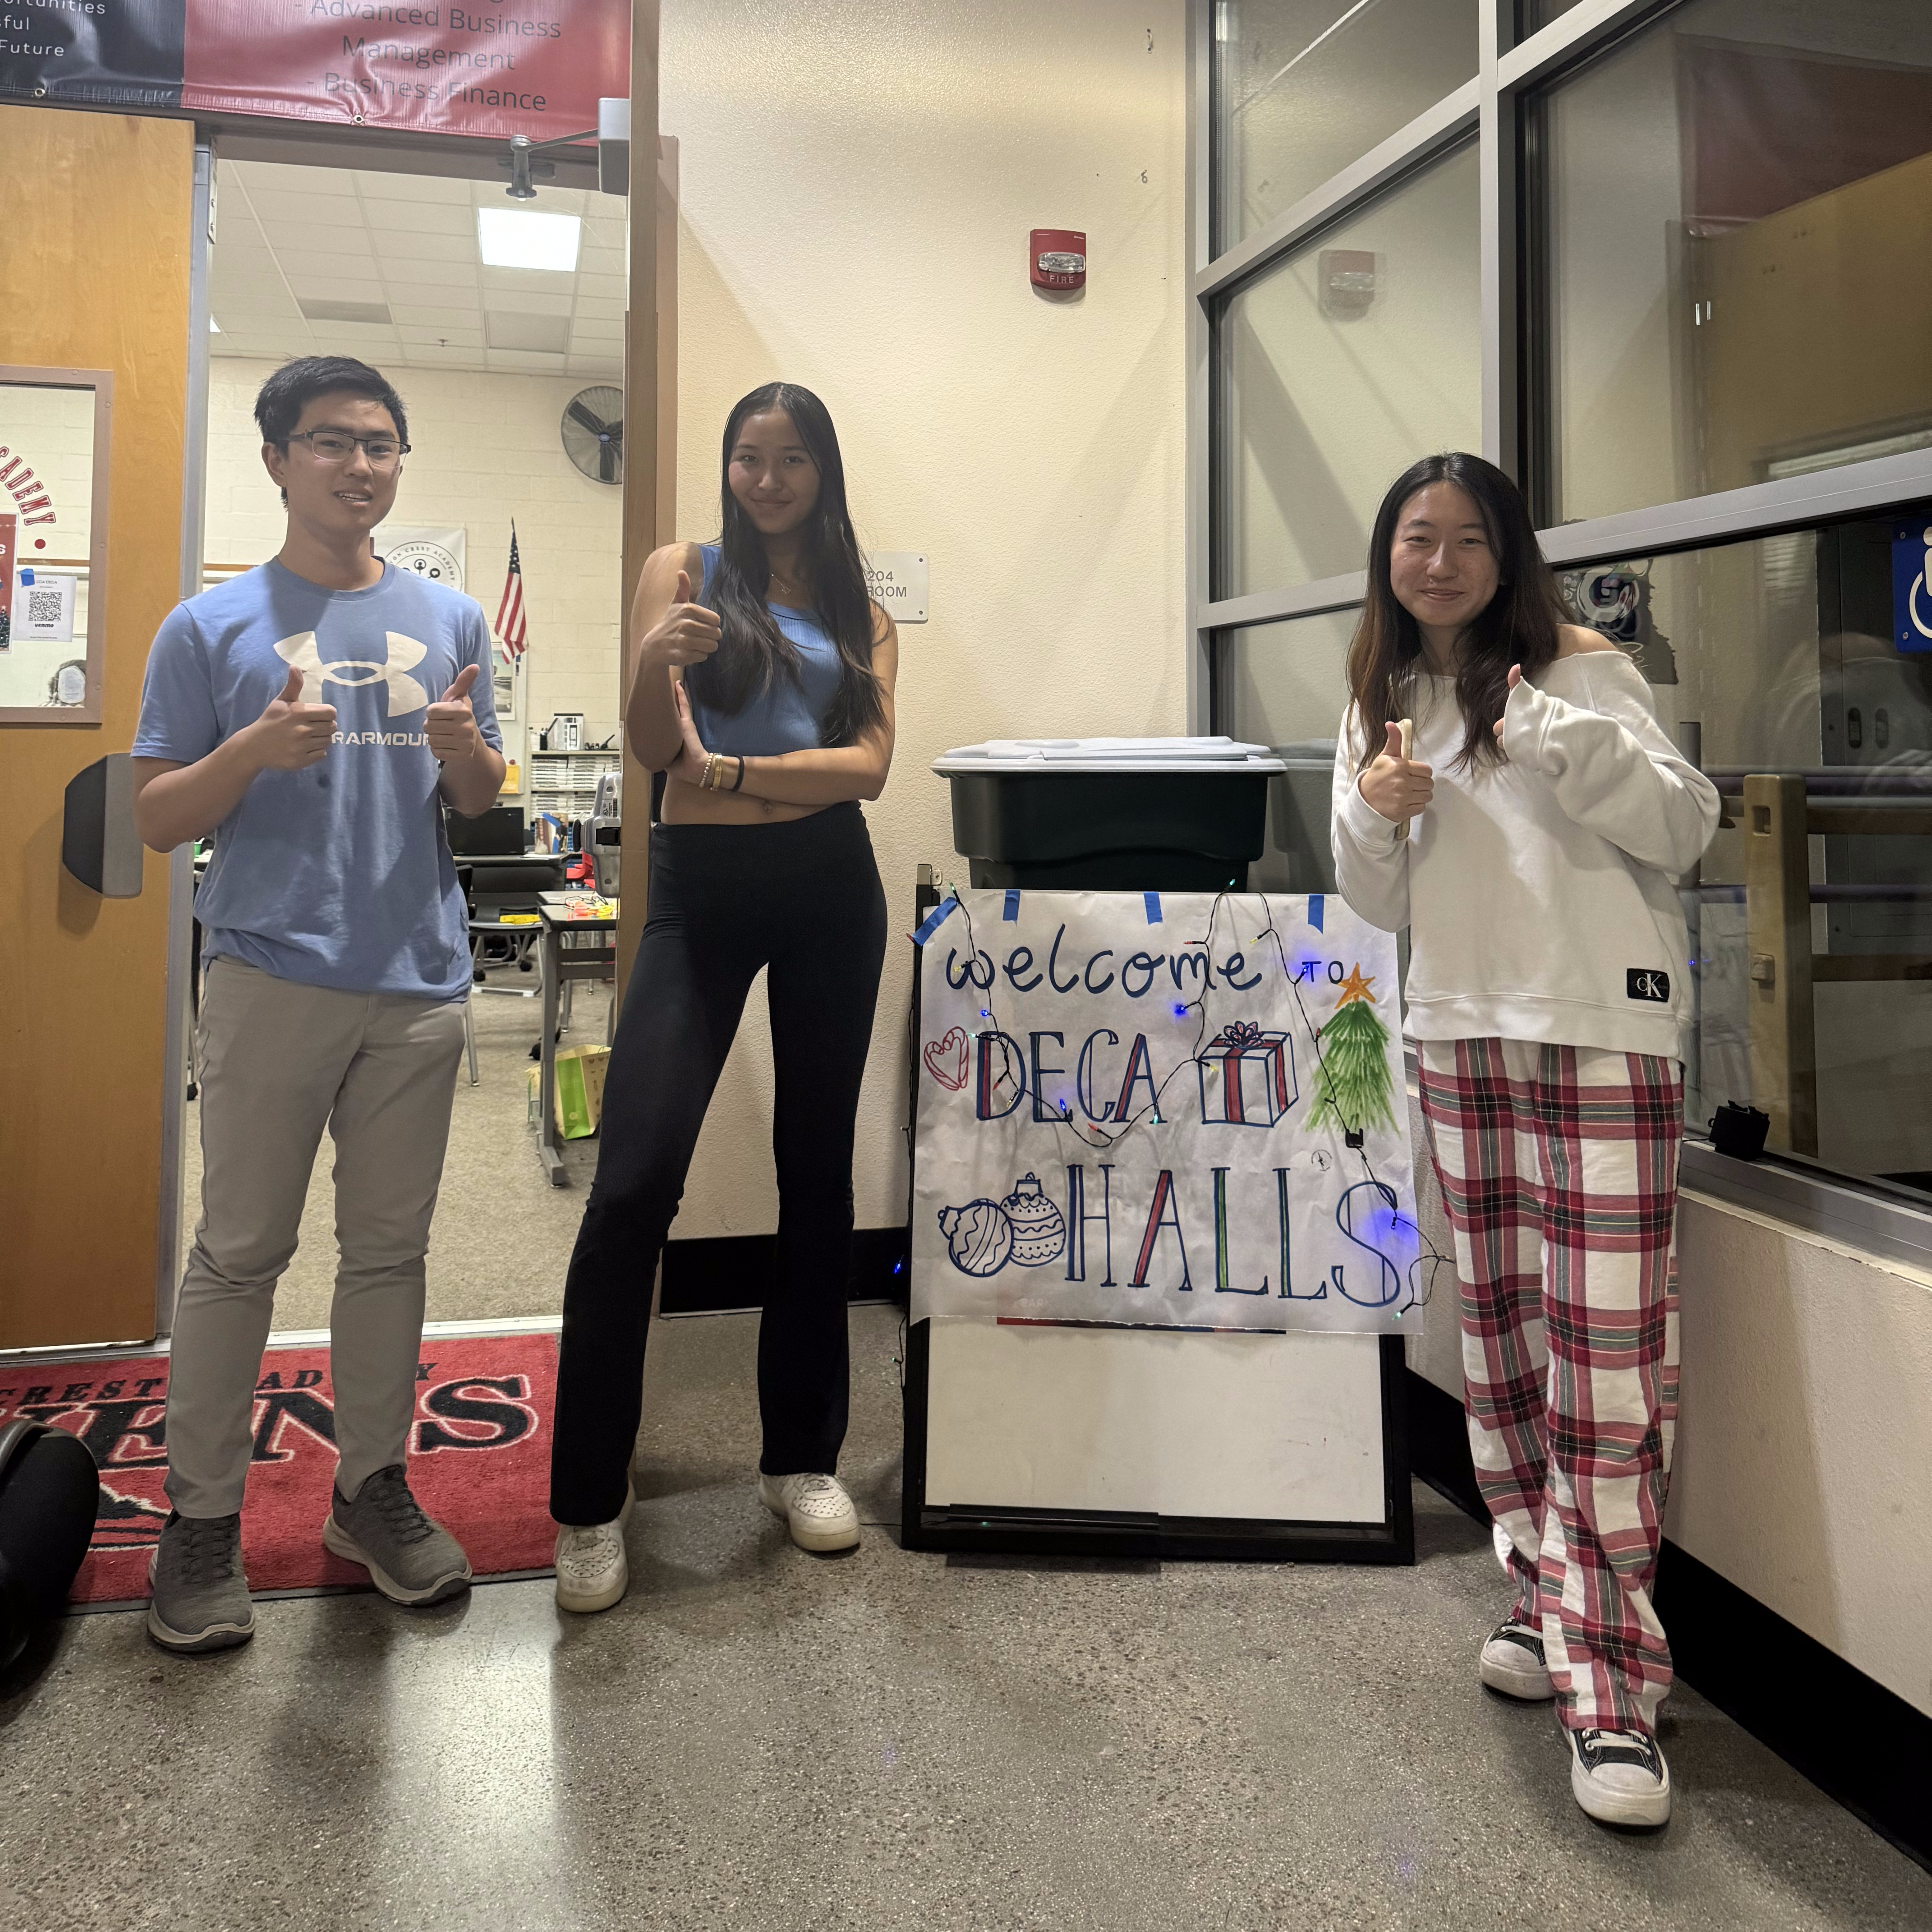
\includegraphics[width=0.28\textwidth]{group.png}
	% \caption{(from left to right) Nathan Dai, Ruby Gao, Lynn Huang}
% \end{wrapfigure}

Our DECA chapter embarked on a fundraising journey with an initial capital of \$210, generously donated by parents through our GoFundMe campaign. We organized a carnival, which, despite a lower-than-expected turnout from AP Statistics students, was a success. The carnival featured a variety of games, including Nerd Nerf Battle Turf, Wheel of Fortune, Chess vs. Wayne, Las Vegas Casino, Steven the Dinosaur, Chopsticks vs. Asian Dad, Tip Jar, and Papa's Ramenria. Detailed rules and a comprehensive list of these games can be found in Appendix \ref{appendix:carnival_games}.

In addition to the games, we also offered hot chocolate and Christmas-themed goodie bags for sale. The carnival raised \$172. Subsequently, we sold our remaining prizes at the Swap Meet and other venues, generating an additional \$205.

We also hosted several food-related fundraisers. Our partnership with Happy Lemon and Chipotle, where a portion of the proceeds from flyer-presenting customers was donated to DECA, resulted in earnings of \$25 and \$71, respectively. On-campus food truck events with Kona Ice and Wetzel Pretzel right after school contributed \$50 and \$165, respectively, to our funds.


\section{Monitoring and Controlling}

\subsection{Monitoring}

Monitoring — describe how you monitored your schedule, budget and project quality

\subsection{Controlling}

Controlling — list issues encountered and how you dealt with them


\section{Closing the Project}

\subsection{Evaluation of Key Metrics}

Evaluation of key metrics

\subsection{Lessons Learned}

Lessons learned — describe what worked well and what didn't work well for each of the project management processes: initiating, planning and organizing, execution, monitoring and controlling

\subsection{Recommendations for Future Projects}

Recommendations for future projects



\clearpage

% Bibliography
\bibliographystyle{IEEEtran}
\bibliography{bibliography/references}{}
% \printbibliography

% Appendix
\begin{appendices}
	\section{Chi-Square Goodness-of-Fit Test}
\label{appendix:chi_square}

The Chi-Square Goodness of Fit Test is a statistical hypothesis test used to determine whether observed frequencies differ significantly from expected frequencies specified in the null hypothesis. It is a non-parametric test that compares the observed distribution of data with an expected distribution, and it is most commonly used with categorical data. The test statistic is calculated as:

$$\chi^2=\sum\frac{(O_i-E_i)^2}{E_i}$$

where:
\begin{conditions}
\chi^2 & the test statistic \\
O_i & the observed frequency of outcome $i$ \\
E_i & the expected frequency of outcome $i$
\end{conditions}

\section{Law of Large Numbers}
\label{appendix:large_numbers}

The Law of Large Numbers is a fundamental concept in probability and statistics. It states that as the size of a sample increases, the sample mean will get closer to the expected value of the population. In other words, the average of the results obtained from a large number of trials should be close to the expected value and will tend to become closer as more trials are performed.

Mathematically, if $X_1, X_2, X_3...X_n$ are independent and identically distributed random variables with expected value $E(X_i)=\mu$, then the Law of Large Numbers is expressed as:

$$\lim_{n\to\infty}\frac{1}{n}(X_1+X_2+...X_n)=\mu$$

\section{Favorite-Longshot Bias}
\label{appendix:favorite_longshot}

The Favorite-Longshot Bias is a phenomenon observed in gambling markets where the expected returns on bets placed on longshots (i.e., outcomes with low probabilities of occurrence) are significantly lower than those of favorites (i.e., outcomes with high probabilities of occurrence). Despite the lower returns, bettors disproportionately favor longshots.

This bias has been documented in various betting markets, including horse racing, sports betting, and lottery games. The bias suggests that bettors tend to overestimate the chances of unlikely events and underestimate the chances of likely events.

While there is no consensus explanation for the favorite-longshot bias \cite{ottaviani_2008_chapter}, several theories have been proposed. Some suggest that it may be due to misperceptions of probabilities, while others attribute it to the utility of gambling (i.e., the thrill of potentially winning a large amount from a small stake).

In the context of a carnival or similar event, understanding this bias can be useful for game organizers. By offering large potential prizes for unlikely outcomes, they can attract more participants and increase overall profits, even if the games are statistically rigged in favor of the organizer. This is because the possibility of winning a large prize can make the risk of losing seem worthwhile to many participants.

\section{Temu Purchase List}
\label{appendix:temu}

\begin{table}[H]
	\centering
	\caption{List of prizes purchased and their respective prices}
	\begin{tabular}{l|rrr}
	\textbf{Item}           & \multicolumn{1}{l}{\textbf{Price (\$)}} & \multicolumn{1}{l}{\textbf{Quantity}} & \multicolumn{1}{l}{\textbf{Total (\$)}} \\ \hline
	Assorted Stickers       & \$ 0.03                                 & 100                                   & \$ 3.00                                 \\
	Fidget Toy              & \$ 0.23                                 & 30                                    & \$ 6.90                                 \\
	Squishy                 & \$ 0.25                                 & 20                                    & \$ 5.00                                 \\
	Boba Keychain           & \$ 1.12                                 & 4                                     & \$ 4.48                                 \\
	Pokemon Painting        & \$ 1.88                                 & 3                                     & \$ 5.64                                 \\
	Hello Kitty Keychain    & \$ 1.99                                 & 3                                     & \$ 5.97                                 \\
	Cat Poster              & \$ 2.28                                 & 3                                     & \$ 6.84                                 \\
	USB Splitter            & \$ 2.48                                 & 3                                     & \$ 7.44                                 \\
	Mini Game Console       & \$ 2.78                                 & 3                                     & \$ 8.34                                 \\
	Slime                   & \$ 2.78                                 & 3                                     & \$ 8.34                                 \\
	Blue Dinosaur Plushy    & \$ 3.59                                 & 2                                     & \$ 7.18                                 \\
	Pink Dinosaur Plushy    & \$ 4.04                                 & 2                                     & \$ 8.08                                 \\
	Strawberry Plushy       & \$ 5.10                                 & 2                                     & \$ 10.20                                \\
	Paws Painting           & \$ 7.48                                 & 1                                     & \$ 7.48                                 \\
	Cherry Blossom Lego Kit & \$ 8.27                                 & 2                                     & \$ 16.54
	\end{tabular}
	\label{tab:temu}
\end{table}

\section{Amazon Purchase List}
\label{appendix:amazon}

\begin{table}[H]
	\centering
	\caption{List of items purchased on Amazon and their respective prices for the goodie bags}
	\begin{tabular}{l|l}
	\textbf{Item}               & \textbf{Cost (\$)} \\ \hline
	Big Candy Canes             & \$    8.99         \\
	Reese's Peanut Butter Trees & \$  12.99          \\
	Ghirardelli Peppermint Bark & \$  14.99          \\
	Christmas Stickers          & \$  10.75          \\
	Chrsitmas Tattoos           & \$    4.62         \\
	Plastic Goodie Bags         & \$    6.45
	\end{tabular}
	\label{tab:amazon}
\end{table}

\section{Costco Purchase List}
\label{appendix:costco}

\begin{table}[H]
	\centering
	\caption{List of items purchased at Costco and their respective prices for the hot chocolate bar}
	\begin{tabular}{l|l}
	\textbf{Item}            & \textbf{Cost (\$)} \\ \hline
	European Cookies         & \$  14.99          \\
	Heavy Whipped Cream      & \$    3.99         \\
	12 oz Cups (100 Ct)      & \$    7.99         \\
	Swiss Miss Hot Chocolate & \$    7.99         \\
	Whole Milk               & \$    3.65
	\end{tabular}
	\label{tab:costco}
\end{table}

\section{Detailed List of Carnival Games}
\label{appendix:carnival_games}

\textit{Nerd Nerf Battle Turf}

This game involves nine balloons, each representing a different prize. Participants are given a Nerf gun and three chances to hit a balloon for a small prize, two chances for a medium prize, and one chance for a large prize.

\textit{Wheel of Fortune}

A classic carnival game where participants spin a fortune wheel. The outcome of the spin corresponds to different prize levels.

\textit{Chess vs. Wayne}

In this game, participants play a game of chess against an individual named Wayne. Winning the game yields a large prize, while losing still grants a small prize.

\textit{Las Vegas Casino}

This game consists of two parts. First, participants choose a color (red or black), then a roulette board is spun and a metal ball is dropped. If the ball lands on the chosen color, the participant advances to the next round. Landing on green yields an automatic big prize. Second, participants choose a cup from ten options (five filled with salt, five with sugar). Selecting a sugar-filled cup wins a small prize.

\textit{Steven the Dinosaur}

This is a card game where participants are given a card from 2-10, while the remaining eight cards are divided into two piles. Each turn, participants guess which card is in each pile. The game ends when an incorrect guess is made or all cards are correctly guessed. The number of correct guesses corresponds to different prize levels.

\textit{Chopsticks vs. Asian Dad}

In this game, participants must move rice from one bowl to another using chopsticks, aiming to beat Ruby's dad's time. This game tests the participant's dexterity and speed.

\textit{Tip Jar}

This game involves adding tickets to one of two jars, representing two characters from the recent Hunger Games movie: Coriolanus Snow and Finnick Odair. People can vote for their favorite character by adding tickets to the corresponding jar.

\textit{Papa's Ramenria}

This game involves guessing a customer's preferred soup base and side dish, and selecting four toppings for their ramen without choosing the one they're allergic to. Correct guesses advance the participant to the next level and yield various prizes, while incorrect guesses end the game.

\section{eBay Transaction Fees}
\label{appendix:ebay_fees}

\begin{table}[H]
	\caption{Sample eBay transaction fees for a \$19.99 item in the \textit{Home \& Garden} category}
		\begin{tabular}{l|l}
		Order   Subtotal                    & \$      21.54        \\ \hline
		Tax                                 & \$    (1.55)         \\
		Order Total                         & \$    19.99          \\ \hline
		Variable Fee (13.25\%)              & \$    (2.85)         \\
		Final Value Fee (fixed per order) & \$    (0.30)         \\
		Shipping (USPS)                     & \$    (3.64)         \\ \hline
		\textbf{Gross Profit}               & \textbf{\$    13.20}
		\end{tabular}
	\label{tab:ebay_fees}
\end{table}

\autoref{tab:ebay_fees} shows the transaction fees for a \$19.99 item sold on eBay. The variable fee is 13.25\% of the order subtotal, and the final value fee is a fixed \$0.30 per order. The shipping cost is \$3.64, and the gross profit is \$13.20.


\end{appendices}

\end{document}
